\documentclass[a4paper,12pt]{article}
\usepackage{amssymb}
\usepackage{geometry}
\usepackage{graphicx}
\usepackage{colortbl}
\usepackage{wrapfig}
\geometry{margin=1in}



\begin{document}

Dustin Kane

CMSI 370-01

November 24, 2015

\begin{center}
\section*{Assignment 1124: Dream Design}
\subsection*{The Ultimate Heads-Up Display with Microsoft HoloLens}
\end{center}

\section{Introduction}
\subsection{A Bicycle For Our Minds}

Steve Jobs, the cofounder of Apple Computers, liked to tell a story. He found a study that measured the distance versus energy consumption for various animals. The study found the condor to be the most efficient animal and put humans fairly far down the list. However, Scientific American decided to test the efficiency of a human on a bicycle. A person on a bicycle was by \emph{far} the most efficient animal on the planet. With that in mind, Steve Jobs said this:

\begin{quote} 
    ``And that's what a computer is to me. What a computer is to me is it's the most remarkable tool that we've ever come up with, and it's the equivalent of a bicycle for our minds.'' - Steve Jobs [1]
\end{quote}

Computers are bicycles for our minds. They are augmentations to our intellect. Or, at least they should be. Computers today do not really achieve this vision. The Scientific American test implied that the bicycle was the extension of a person; a person \emph{on} a bicycle \emph{is} the most efficient animal. A modern computer is not an extension of a person. It is a tool: an interface that a person has to interact with. A computer is more like a parking meter or a cashier at a store; it isn't an extension of the person using it by any stretch of the imagination. Smart phones feel more like an extension of a person; people are tethered to their phones and sometimes filter every thought and action through it. But the way they interface with it is still like the way they interact with a garage-door opener or a television remote. Computers are incredibly useful, but their interfaces are essentially just consoles: a set of buttons and switches that make the machine do something. To create an interface that lives up to the dream of the Bicycle of the Mind, we need an interface that we feel connected to and integrated with.

\subsection{Realizing the Mind-Bicycle Dream}
To put it in more concrete terms, a bicycle takes the existing human behavior of movement and improves it by making it faster and more efficient. A computer should take existing human mental behavior and improve it by making it faster, more efficient, and even more. Instead of giving you turn-by-turn directions through Google Maps, the computer should improve your ability to \emph{know} where to go. Instead of allowing a user to look up an actress on IMBD, a computer should improve the ability of the user to \emph{remember} what movies she was in. Instead of providing the user with a calculator, the computer should improve the ability of the user to \emph{calculate} arithmetic problems. I'm not suggesting the computer augment the brain to be more effective; that would be like suggesting a bicycle allows a man to move his legs faster. The problem is the way we interact with computers is more akin to the way we interact with a servant or a secretary: we ask it questions and we give it commands. We do not interact with a bicycle by telling it to go faster: we interact with a bicycle by moving our legs in a way that is fairly similar to the way we would move them without the bicycle, and the bicycle augments that behavior. In the same way, we should interact with a computer by, essentially, doing what we do without a computer and the computer handles the rest.

I imagine a computer that, instead of a screen, superimposes information on our field of vision through a pair of glasses. The computer sees what we see and hears what we hear. We give the computer instructions by, essentially, thinking out loud. Just like we slightly alter the motion of running to apply it to a bicycle, we slightly alter our way of thinking to apply it to this interface. I believe this kind of interface could be created today using the existing concept of a ``Heads-Up Display'' [2] and implementing it with the Microsoft HoloLens hardware [4].

\section{The Heads-Up Display}

\subsection{Heads-Up Displays in Military Aircraft}

\begin{wrapfigure}{r}{0.5\textwidth}
\centering
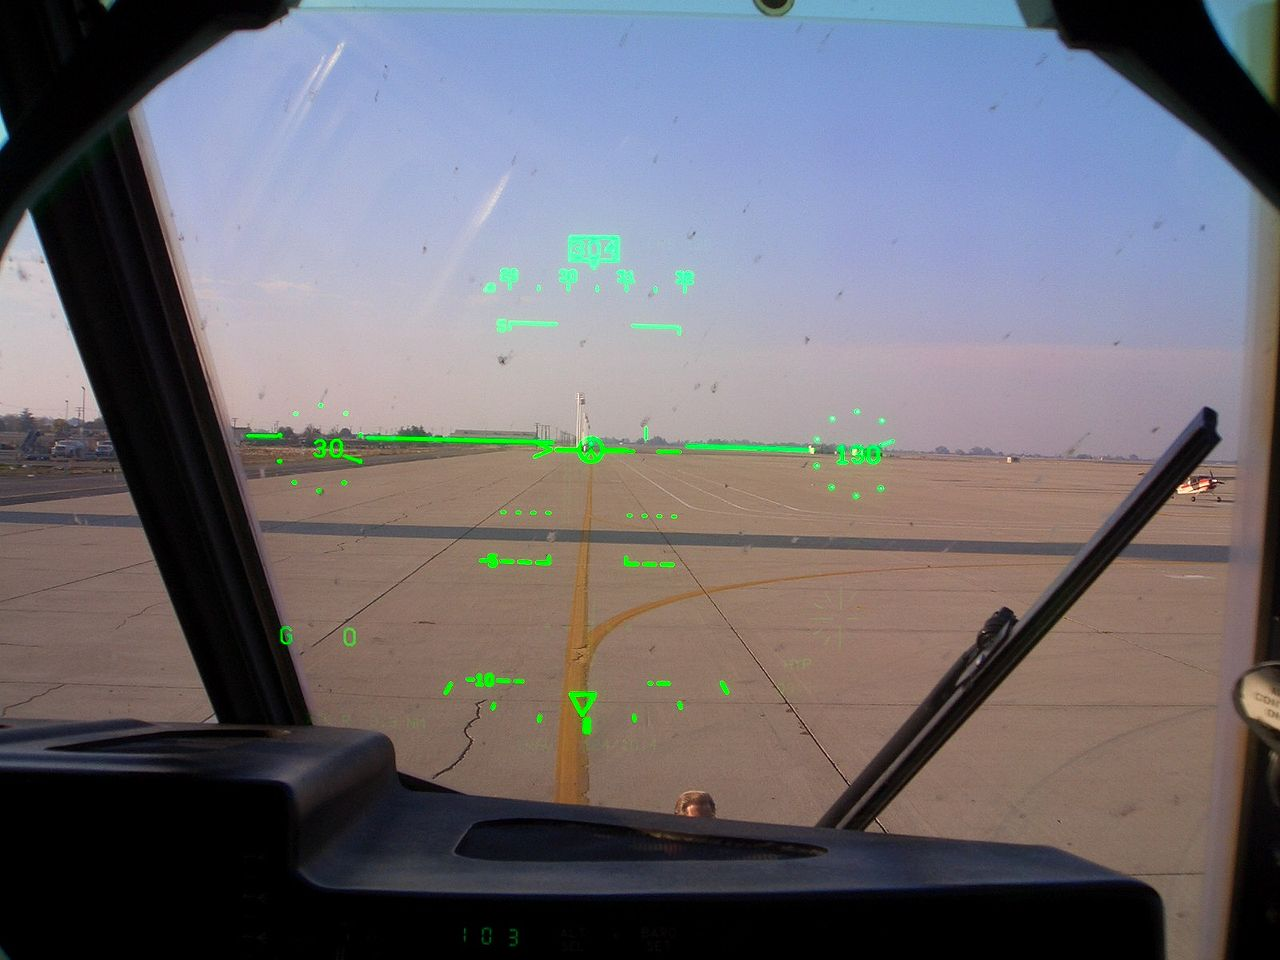
\includegraphics[width=0.5\textwidth]{jethud}
\caption{HUD of a C-130J [3]}
\end{wrapfigure}

A Heads-Up Display is a kind of instrument that super-imposes information over what the user would otherwise be looking at. This kind of instrument is mostly used in military aircraft. The fighter jet has a transparent screen in the cockpit between the pilot and the front windshield. The pilot can now look at readings from his instruments while looking straight ahead; he doesn't have to look down at his instruments, he keeps his head up, hence the name Heads-Up Display.

This interface does more than save the pilot from having to move his head. Like the bicycle, the jet is meant to be an extension of the human being. The pilot looks straight forward at where he's flying. With the Heads-Up display, instead of interacting with his instruments in a kind of transactional way---looking down at them, querying them for information---the pilot has the relevant information right in front of him. The action of the pilot is the same as if the instruments weren't there, yet he still gets the benefit of having the information from them. His ability to fly is augmented by the availability of the information from the Heads-Up Display.

\subsection{A Heads-Up Display For Everyday Life}

The dream interface takes the Heads-Up Display out of the fighter jet and into the hands of the average person. Instead of displaying altitude and air speed, the Heads-Up Display can display turn-by-turn directions, restaurant reviews, news articles, and more. Instead of looking down at a phone for directions, or listening to a voice say to ``use the second lane to turn right onto the Christopher Columbus Transcontinental Freeway I-10,'' the user can look, straight ahead, at where they are going with an arrow showing them exactly what lane to drive in and what direction to go in. Here, the interface allows the user to behave as if they already knew where they were going. Then, a breaking news banner could scroll across their view telling them there has been a terrible accident somewhere. Here, the interface allows the user to behave as if they were really well informed; they didn't actively seek out the news, they act as if they already knew it.

\subsection{Augmented Reality}


Similar types of interfaces already exist, and they go by the name \emph{augmented reality}. 
\begin{wrapfigure}{l}{0.5\textwidth}
\centering
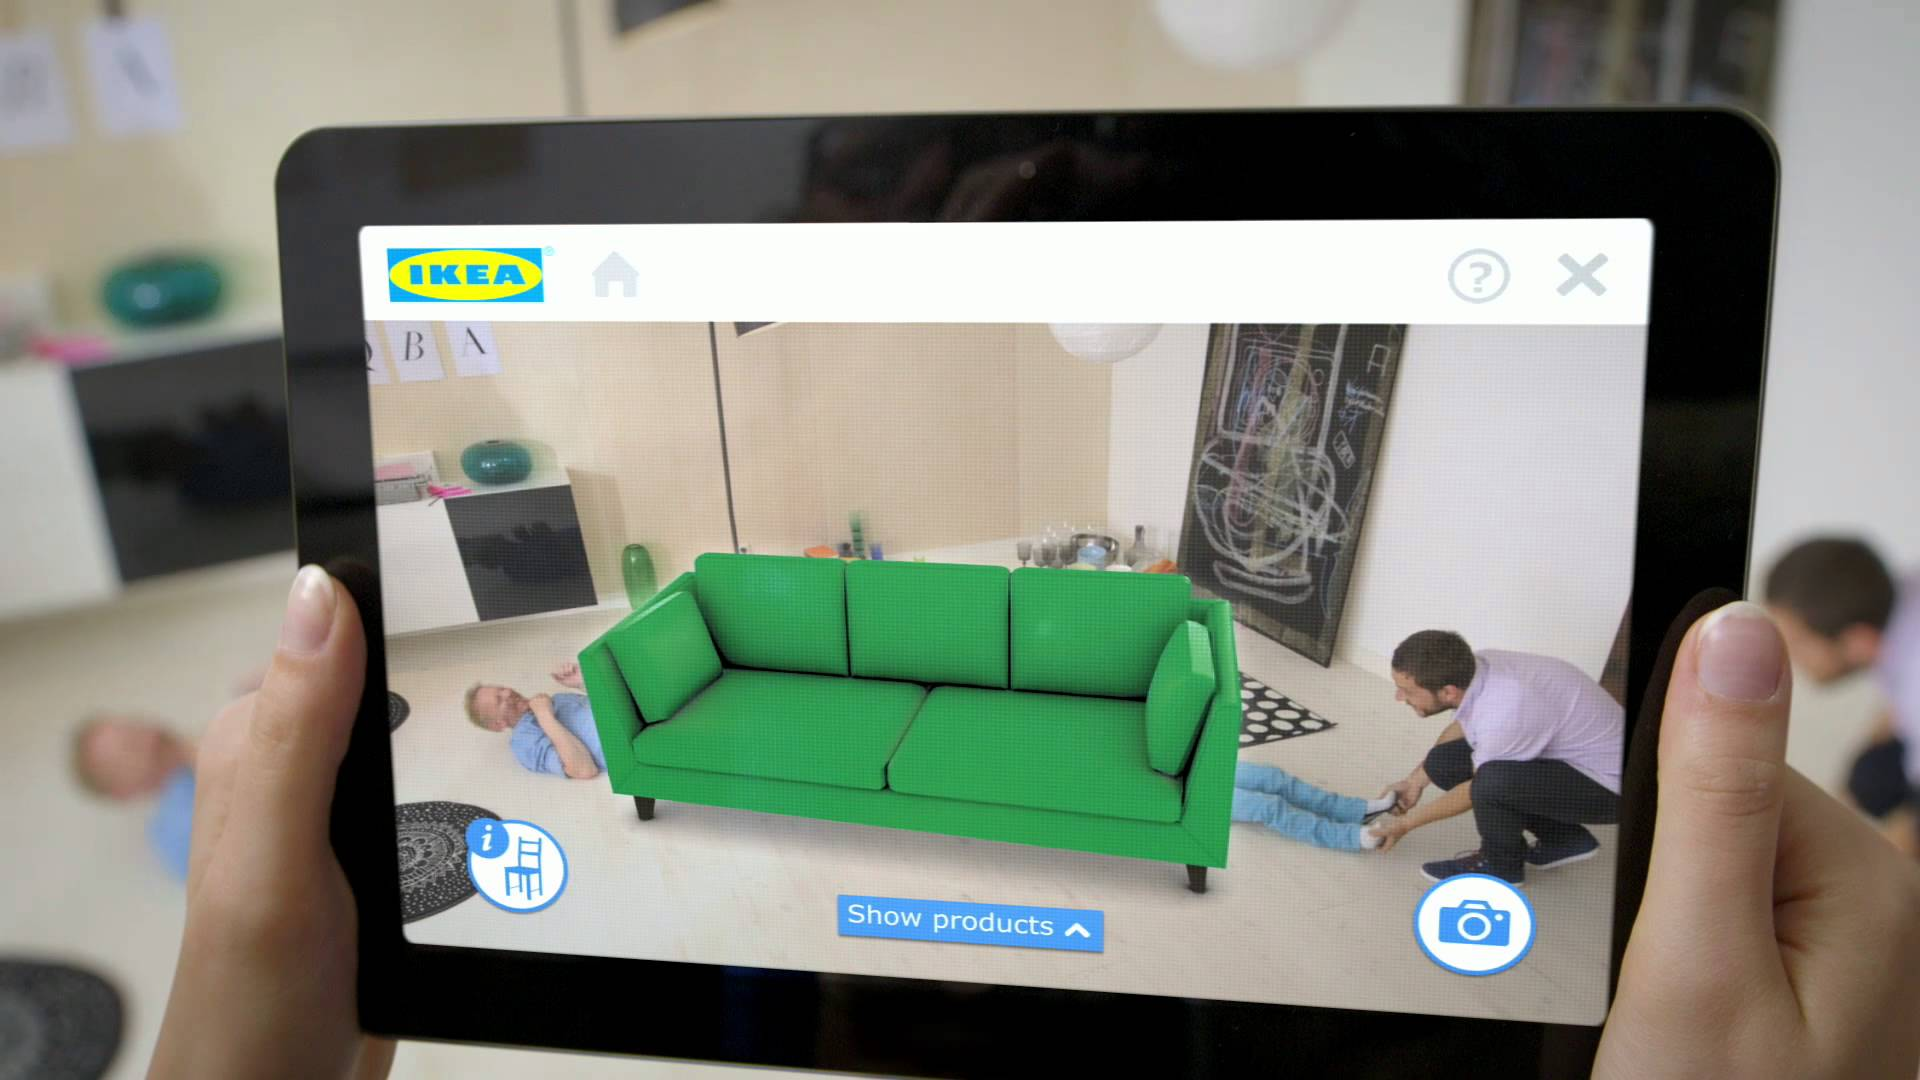
\includegraphics[width=0.5\textwidth]{ikea}
\caption{IKEA Catalog app [5]}
\end{wrapfigure}


Augmented reality refers to computers ``augmenting'' the real, physical world [4]. Figure 2 shows the IKEA Catalog app [5]. This app allows you to use your mobile device's camera to see what a room would look like with IKEA furniture. The app overlays the computer-generated furniture onto the image from the camera. The furniture is manipulable using the touch screen of the device. This is a favorable interface because it enhances something the user already does without a computer: visualizing how furniture will look in a room. This is something a user would, otherwise, do with their imagination. Technology comes in and creates the actual image to create a more accurate depiction of what the furniture will actually look like.

\begin{wrapfigure}{r}{0.5\textwidth}
\centering
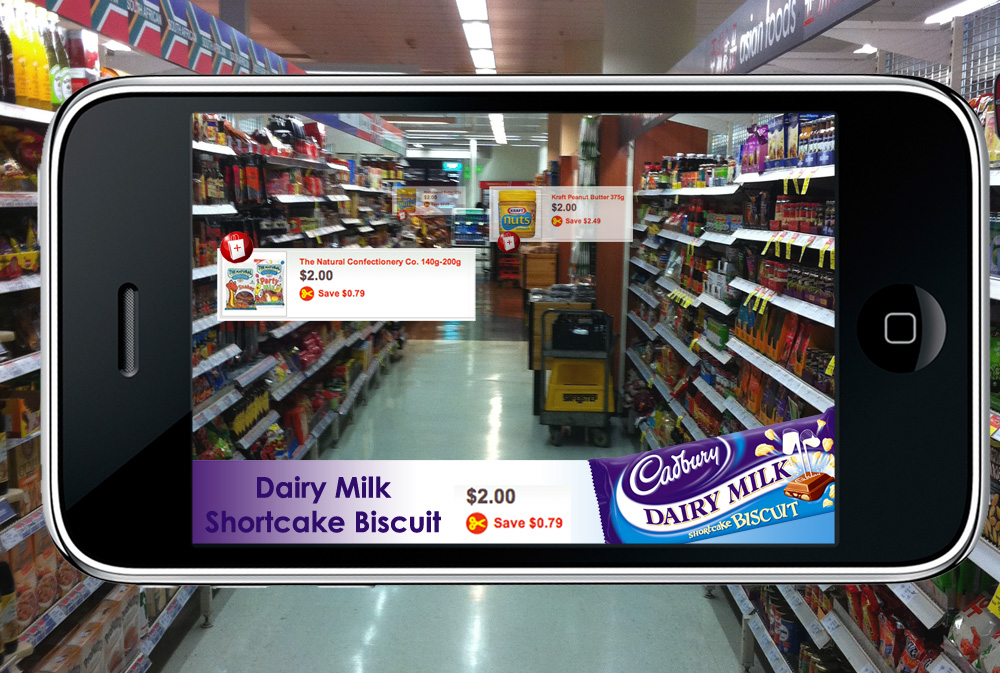
\includegraphics[width=0.5\textwidth]{coupons}
\caption{This app displays coupons and pricing for items at a grocery store [6]}
\end{wrapfigure}

Figure 3 provides another example. This app shows the user coupons and alternate prices for items at a grocery store. The user points their phone's camera at items at the store and the app overlays prices and coupons next to the items in the image. This is a better interface than searching for prices online because it enhances the user's knowledge of prices. Instead of asking a third party, the user is presented the information next to the items in their view. The user behaves as if they knew the prices already, but they are actually being supplied with the beneficial information by the computer.

Matthew Buckland wrote an interesting essay on the potential applications of augmented reality to social networking [7]. Illustrated in Figure 4, Buckland imagines an interface where the user can hold up their phone's camera to a row of houses and get various data from social media. The data may include information about an upcoming block party, or a location on a map. It could also have tags next to each house representing profiles of each resident with quick buttons to get in contact with each of these people. Here, the computer is enhancing the user's ability to recognize houses and the people who live in them. It's also incredibly efficient because it includes interactive buttons for things like messaging right next to the houses in the image. This example is the most similar to the interface I'm proposing.

\begin{figure}
\centering
\includegraphics[width=\textwidth]{social}
\caption{A concept design of an augmented reality app centered around social media [7]}
\end{figure}

There is a problem with each of these examples, however. In Figures 2-4, there is a visible device. For this interface to reach its full potential, there cannot be a visible device. First, the edges of the device obstruct the user's view; in Figure 3 we cannot see what items are behind the black bars of the iPhone. Second, the entire field of view is not augmented by the interface; users have to look at the world through their device, either holding it uncomfortably close to their face or getting a very small porthole to see the augmented world. Finally, the user's hands aren't free. The user must hold the device up, making them unable to use their hands in ways they normally would. This interface would be impossible to use for getting directions while driving, or instructions while cooking, for example. For this interface to realize its potential it must include the user's entire view, it must not obstruct any part of the user's view, and it must be hands free. 



\section{The Microsoft HoloLens}

\subsection{The Augmented Reality Device}

In January 2015, Microsoft unveiled the HoloLens, a device designed for augmented reality [9]. The HoloLens is a headset that displays images on a transparent screen right in front of the user's eyes. Unlike many \emph{virtual reality} headsets released prior to it that create an \emph{entirely} virtual world, the HoloLens is transparent and lays computer-generated images over the user's view of the real world. As Microsoft puts it on their website: 

\begin{quote}
``Microsoft HoloLens generates a multi-dimensional image visible to a user so that he or she perceives holographic objects in the physical world. Holographic objects seen with Microsoft HoloLens can be placed in physical locations you choose, move according to their own rules, or remain in a specific location within your field of view regardless of where you are or in which direction you are looking.'' - Microsoft [10]
\end{quote}

\subsection{What Can It Do?}

The key feature of the HoloLens is that, through its sensors, and complex processor, it can react to user gestures. As Microsoft puts it: 

\begin{quote} 
    ``The holograms you'll see with Microsoft HoloLens can appear life-like, and can move, be shaped, and change according to interaction with you or the physical environment in which they are visible. Use gestures to create, shape, and size holograms. Use your gaze to navigate and explore. Use your voice to communicate with your apps. Microsoft HoloLens understands your movements, gaze, and voice, enabling you to interact with content and information naturally. Using holograms, you can place your digital content, such as apps, information, and even multi-dimensional videos, in the physical space around you, so you can interact with it.'' - Microsoft [10]
\end{quote}

The idea is the HoloLens can create virtual objects that can be manipulated by the user. It can sense the user's hands and recognize gestures to allow for things like moving and interacting with objects. It also immerses the user in computer-generated images, using their entire field of view. 

It is able to do this with dedicated hardware. Microsoft says

\begin{quote}
    ``The HPU is custom silicon that processes a large amount of data per second from the sensors. Microsoft HoloLens understands gestures and where you look, and maps the world around you, all in real time.'' - Microsoft [11]
\end{quote}

Though Microsoft has only released a limited amount of detailed information about the device and how it works, based on live demos of users playing various video games and interacting with 3D models (all viewable on the HoloLens product page [12]), we can assume the device is fairly robust in its computing capabilities for things like image projection and complex gesture recognition. 

\section{The Dream Design: An Interactive Heads-Up Display with Microsoft HoloLens}

\subsection{Putting It All Together}

My dream design, essentially, takes the interface in Figure 4 and puts it in the Microsoft HoloLens. Instead of looking at the houses through the phone, the user wears the headset and has their reality augmented by the various data and interface elements. But the key element of this design, however, is that the user interacts with it via gestures. In the app in Figure 4, the user can call a friend by hitting the phone icon next to their picture. Since my dream design eliminates the screen of the device, they cannot use the button in this way. However, in my design, the user can still press this button by pressing the button they see. Figure 5 is a (crude) illustration of this interface. The user is walking down a street and they can see Yelp reviews of nearby restaurants right before their eyes. Each review has a button to get directions to the restaurant. The user simply points at the button and the interface begins route guidance with arrows along the pavement guiding them.

The user could pull up apps and windows via pressing on short cuts on a kind of ``desktop''. The dream design would also automatically open apps using image recognition. When the user sees a restaurant, the dream design would bring up reviews for that restaurant on Yelp. When the user sees a movie poster, the dream design would bring up the IMDB page for the movie, or recent news.

For more complex commands, the dream design could also incorporate a kind of ``on-screen keyboard''. The interface projects a standard QWERTY keyboard over the user's field of view and they could point to individual letters to ``type''. 

\begin{figure}
\centering
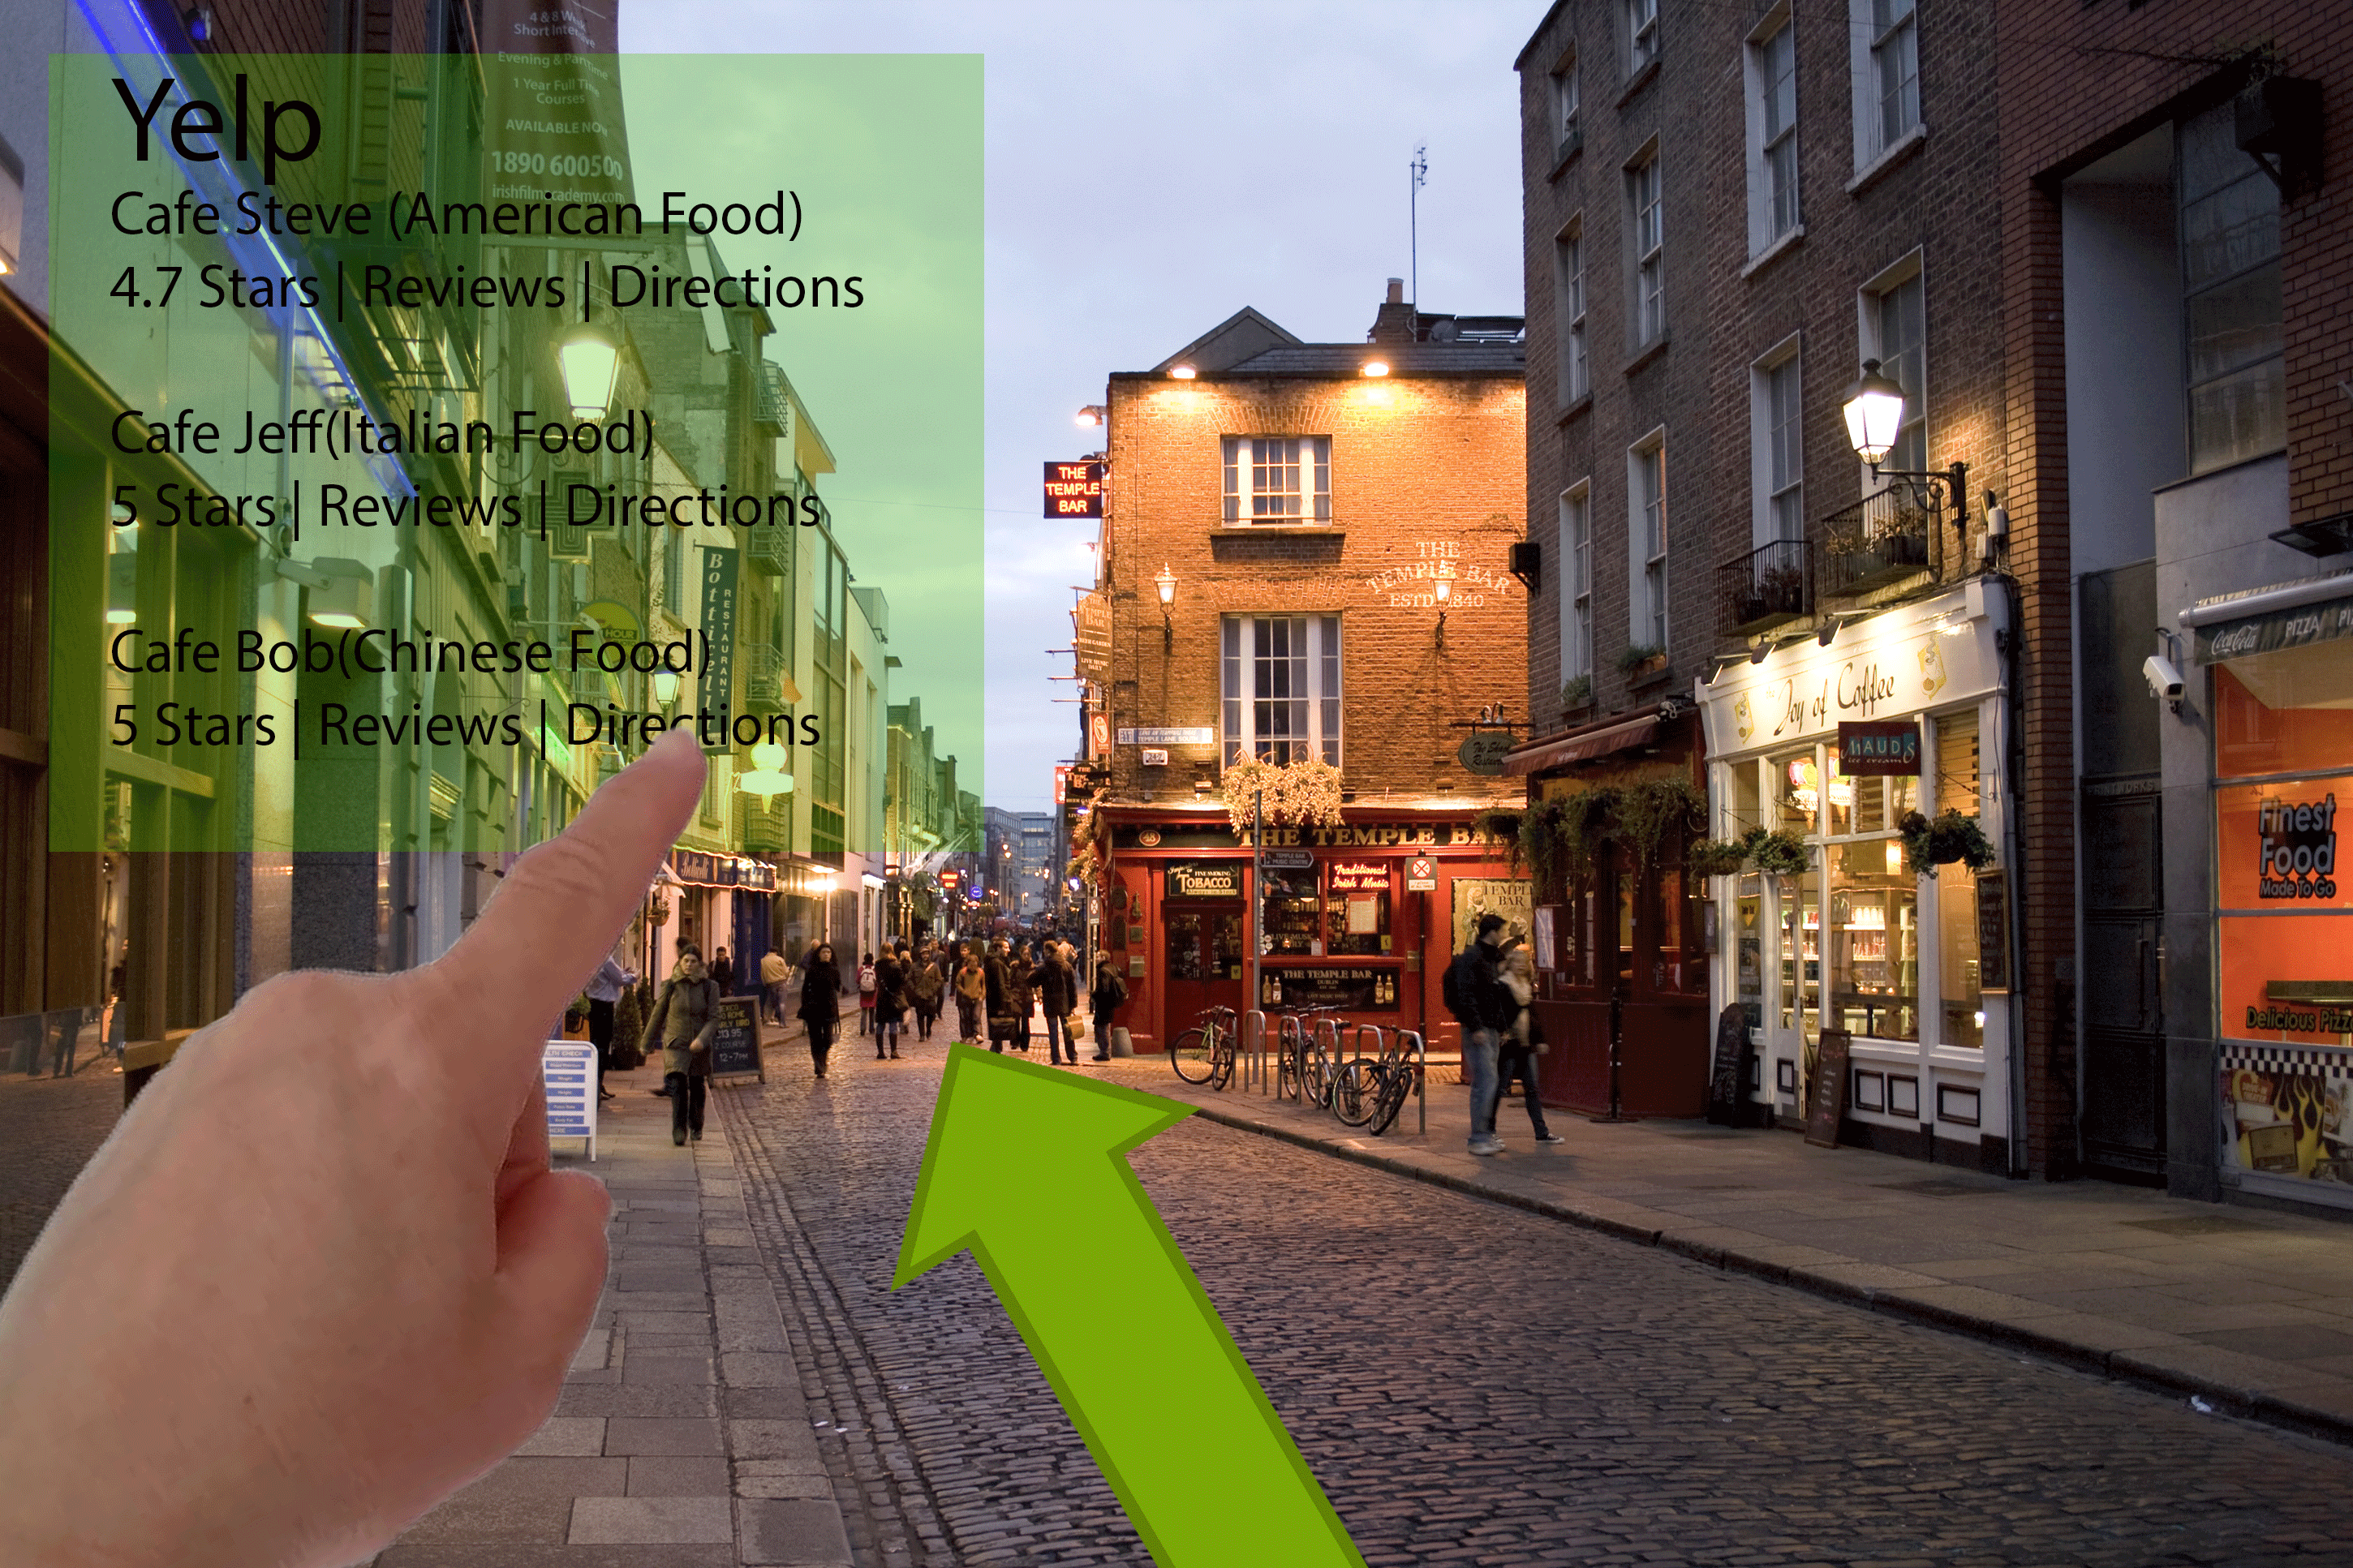
\includegraphics[width=\textwidth]{usage}
\caption{A crude mock-up of my ``Dream Design''. Street image credit [13]}
\end{figure}

\subsection{This Is Possible With Existing Technology}

From what we know about the Microsoft HoloLens, this functionality is completely reasonable. The HoloLens allows the users to manipulate virtual objects with their hands; this requires significantly more sophisticated software than that needed to recognize a finger merely \emph{pointing} to a virtual object. We also know the HoloLens can project complex virtual objects onto the world around the user, like objects on tables; displaying a simple green arrow lining the pavement cannot be more complicated than placing a complex 3D object on a surface.

Assuming the robust capability of the HoloLens to detect gestures, the Dream Design could incorporate direct manipulation interface elements found in desktop applications. The user could change the size of the Yelp ``window'' by pinching the corners and stretching it out. The user could also swipe it away or hit a familiar X in the upper corner. At its absolute simplest, the Dream Design could be, essentially, just a conventional two-dimensional desktop environment displayed over the world via the HoloLens with the tip of the user's finger as the conventional mouse cursor. But the design can be extended far beyond familiar computer interfaces to integrate more closely with the user's world. It can make use of three dimensions by incorporating apps like the IKEA catalog or three-dimensional direction arrows via Google Maps. 

\section{Usability}

To discuss how usable this Dream Design would actually be, I will discuss how the design would likely fare in each of Jakob Nielsen's five Usability Metrics [14]: learnability, efficiency, memorability, errors, and satisfaction. I believe the design would be highly learnable and memorable. The design would vary in efficiency over different tasks and different implementations of apps. It could potentially have a high error rate because the interface is \emph{too} intuitive. Finally, though this metric is subjective, I suspect the interface will be \emph{highly} satisfying to use because its integration would be so seamless in the user experience.

\subsection{Learnability}

Learnability is a metric that answers the question ``How easy is it for users to accomplish basic tasks the first time they encounter the design?'' [14]. I believe this interface will be highly learnable because interacting with it will mimic the way users interact with the real world. Short of mind-reading, this interface could be the most learnable interface possible, because the user literally points at what they want. Humans intuitively use their hands and fingers to point at things. A person learning to use a desktop computer for the first time often points to things on the screen before the person instructing them explains how the mouse works. Since most of the interaction with the interface would be through pointing and ``clicking'' (more apt terminology like ``pressing'', ``touching'', or simply ``pointing'' would likely be necessary), the user would be able to easily figure out how to point at things to interact with the system. 

There would be other elements necessary for the user to learn, such as returning to their list of apps, opening and closing apps, pulling up the on-screen keyboard, and other specific operating system interactions. However, since the experience would be so integrated and service based, there would be very few operating system commands such as switching apps that could be presented in a very straightforward way with buttons depicting familiar symbols, likely out of the way in one of the corners of the user's view.

\subsection{Efficiency}

Efficiency is a metric that answers the question ``Once users have learned the design, how quickly can they perform tasks?'' [14]. Efficiency is where this design would be most lacking. Since the core functionality of the interface is based on simple input like pointing and simple gestures, input will either require strings of many points and gestures, or the command space will be very limited to only allow for certain modes of interacting. This limitation would not be necessarily bad because many of the use cases do not require input: most use cases just involve displaying information. However, apps will either have to have very limited functionality, organize their capabilities through a hierarchy of many buttons the user must navigate through, or make use of the on-screen keyboard, which would likely be hard to type on quickly. Consider an app like Yelp. Yelp could limit its functionality to have no input: it gives you reviews when you see a restaurant. However, one of the key uses of Yelp is \emph{finding} restaurants to go to, so they would want to have a button to find nearby restaurants. However, a Yelp user often wants to filter by price, food type, distance, and other factors, so those must all be buttons. Also, Yelp is not limited to only restaurants, so it must now have more buttons to allow the user to select which kind of establishment they are looking for. Suddenly the user is traversing a maze of buttons to get what they want. The app could also mimic the current Yelp website and require the user to search by typing keywords, but now the user has to use the on-screen keyboard.

\subsection{Memorability}

Memorability is a metric that answers the question ``When users return to the design after a period of not using it, how easily can they reestablish proficiency?'' [14]. Like learnability, memorability will be incredibly high with this interface because there will be very little to remember. Pointing is so intuitive that the user may even do it without remembering that is the actual intended way of interacting with the system. Also, much of it will be automatic based on image recognition and just display information, so remembering how to use the interface is somewhat irrelevant; the user only needs to remember how to read.

\subsection{Errors}

Errors is a metric that answers the question ``How many errors do users make, how severe are these errors, and how easily can they recover from the errors?'' [14]. Errors as a usability metric have a subtle and specific definition: an error is when the user does a deliberate action expecting a result, and the system produces a different result. On the one hand, errors will be incredibly low with this design because it is hard for a user to mess up pointing. The interface is designed to mimic the way humans interact with the world outside of computers very closely. If it achieves this goal, the user's natural inclination when interacting with the design will do exactly what they expect. Pointing at things will select them, grabbing things by the corner and dragging them will move them, pinching the corners of things and stretching them will resize them. On the other hand, however, since we're treating the user interface elements as if they are real-life entities, the user will try to interact with them in all the ways they interact with the real world. Traditional computers benefit from only having a mouse cursor to interpret: this interface will have a complex set of hands. Certain things the user will want to do will simply not be implemented. The user may come up with gestures that haven't been programmed in that they can do to real things---gestures like throwing, waving, and making various shapes with the hands and fingers. We cannot know until we put the system in front of people, but I suspect users will find ways to interact with the interface that weren't considered by the developers.

\subsection{Satisfaction}

Satisfaction is a metric that answers the question ``How pleasant is it to use the design?'' [14]. Hopefully, this is the interface's most successful usability metric. The motivation behind this entire design is to make something that the user feels connected to. They should feel like this computer system is like an article of clothing, or a pair of glasses, or sunscreen. They should feel like the augmentations are not just seamless, but actually benefit their lives. If this design achieves its mission, it should be incredibly fun, natural, and satisfying to use.

\section{Conclusion}

This is not science fiction. All the hardware discussed in this paper currently exists. Interfaces similar to this, and even more complex, also already exist. This is a completely feasible dream. But what I have described is merely a stepping stone. I've tried to combine traditional and familiar user interface concepts and the idea of augmented reality. I described windows, desktop environments, keyboards, and other things found in normal computers. But these are all crutches. They are very useful for interacting with computers as we know them today, but a computer that is integrated in the user's life, that is an extension of them instead of an external servant, would likely have user interface elements that we have never seen before. These elements I previously described lend themselves to traditional computers. I suspect as augmented reality evolves, we will find interfaces that transcend buttons, shortcuts, and links, and is really more similar to how the world actually works.

Until then, however, I feel this design would bring us closer to creating the Bicycle of the Mind. Steve Jobs included a mouse on the Macintosh because he knew the user would want to \emph{point} at the things they wanted to interact with. This dream design takes that design philosophy closer to its logical conclusion. 

\section{Sources}


\begin{enumerate}
    \item https://www.brainpickings.org/2011/12/21/steve-jobs-bicycle-for-the-mind-1990/
    \item https://en.wikipedia.org/wiki/Head-up\_display
    \item https://en.wikipedia.org/wiki/Head-up\_display\#/media/File:C-130J\_Co\_Pilot\%27

    s\_Head-up\_display.jpg
    \item https://en.wikipedia.org/wiki/Augmented\_reality
    \item https://www.youtube.com/watch?v=vDNzTasuYEw
    \item http://augmentedpixels.com/wp-content/uploads/2013/11/augmented-reality-

    marketing.jpg
    \item http://matthewbuckland.com/?p=1041
    \item http://www.matthewbuckland.com/wp-images/futureofsocialnetworking02.png
    \item http://www.theverge.com/2015/1/21/7867593/microsoft-announces-windows-

    holographic
	\item https://www.microsoft.com/microsoft-hololens/en-us/faq
	\item https://www.microsoft.com/microsoft-hololens/en-us/hardware
    \item http://www.microsoft.com/microsoft-hololens/en-us
    \item http://www.bankingtech.com/files/2013/01/high-street-scene.jpg
    \item http://www.nngroup.com/articles/usability-101-introduction-to-usability/
\end{enumerate}


\end{document}